\documentclass{beamer}
\title{EMQX File Transfer}
\author{Ilya Averyanov, Andrew Mayorov}
\institute{EMQX}
\date{2023}
\usetheme{emqx}
\usepackage{listings}
\usepackage{color}
\usepackage{graphicx}
\usepackage{xcolor}
\usepackage{hyperref}
\definecolor{href}{rgb}{0,0,0.9375}
\hypersetup{
    pdfborderstyle={/S/U/W 1}, % underline links instead of boxes
    colorlinks=true,
    urlcolor=href
}
\lstset{frame=tb,
  aboveskip=3mm,
  belowskip=3mm,
  showstringspaces=false,
  columns=flexible,
  basicstyle={\small\ttfamily},
  numbers=none,
  numberstyle=\tiny\color{gray},
  keywordstyle=\color{blue},
  commentstyle=\color{dkgreen},
  stringstyle=\color{mauve},
  breaklines=true,
  breakatwhitespace=false,
  tabsize=2
}


\begin{document}

\frame{\titlepage}

\begin{frame}
    \frametitle{File Transfer}
    \framesubtitle{Idea}

    \begin{center}
        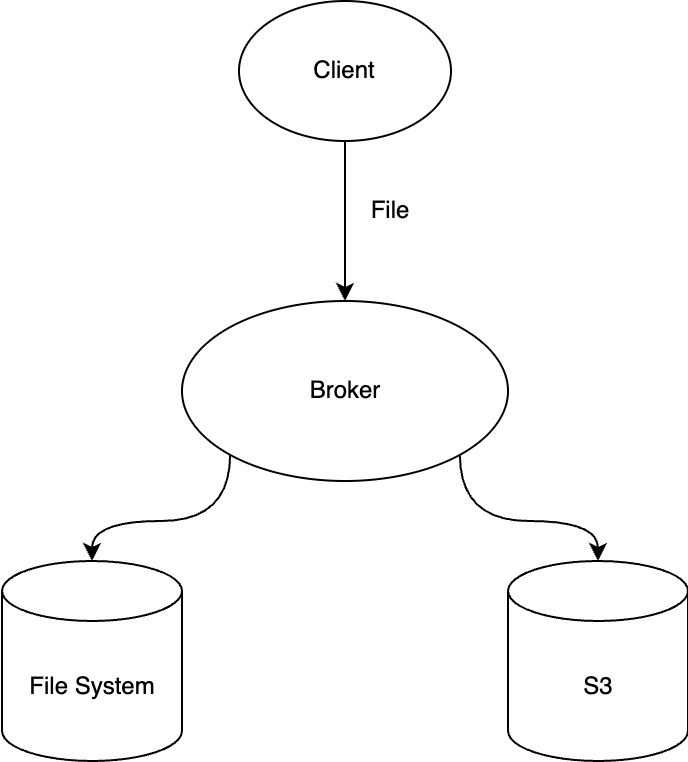
\includegraphics[width=5cm, keepaspectratio]{images/idea.png}
    \end{center}
\end{frame}

\begin{frame}
    \frametitle{File Transfer}
    \framesubtitle{Constraints}

    \begin{center}
        \begin{itemize}
            \item \href{https://github.com/emqx/eip/blob/main/active/0021-transfer-files-over-mqtt.md}{EIP 21}
            \item Over MQTT
            \item Chunked
            \item No additional connections from client
            \item No subcription to special topics
            \item Resumable
        \end{itemize}
    \end{center}
\end{frame}

\begin{frame}
    \frametitle{File Transfer}
    \framesubtitle{Protocol}

    \begin{center}
        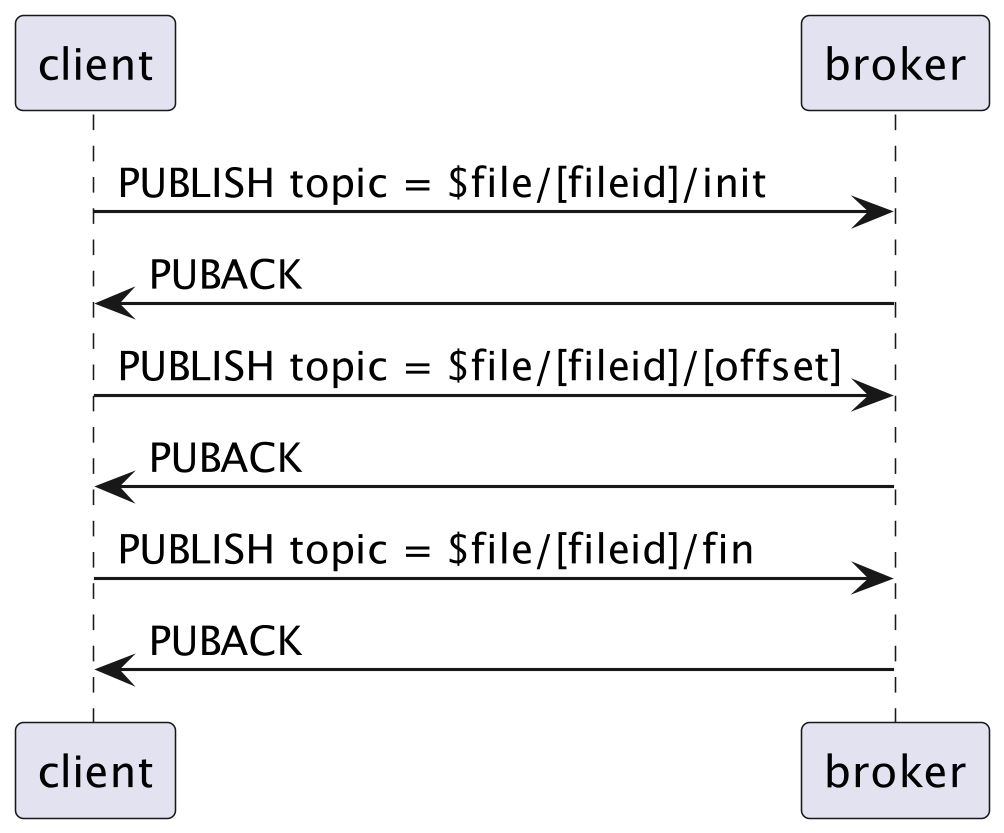
\includegraphics[width=7cm, keepaspectratio]{images/proto.png}
    \end{center}
\end{frame}

\begin{frame}
    \frametitle{File Transfer}
    \framesubtitle{Challenges}

    \begin{center}
        \begin{itemize}
            \item Avoid storing data and even metadata in Mnesia
            \item Cope with clients migrating between nodes
            \item Cope with potentially long-running operations (involving disk and network I/O)
            \item Be minimally invasive*
        \end{itemize}
    \end{center}
\end{frame}

\begin{frame}
    \frametitle{Challenge 1: Avoid Mnesia}

    \begin{center}
        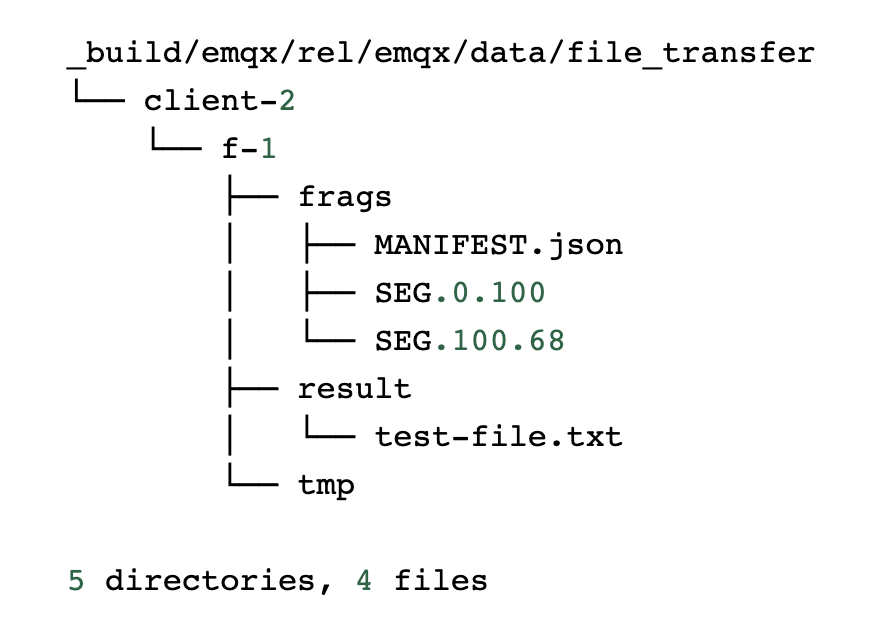
\includegraphics[width=7cm, keepaspectratio]{images/fs-structure.png}
    \end{center}
\end{frame}

\begin{frame}
    \frametitle{Challenge 2: Migrating clients}

    \begin{center}
        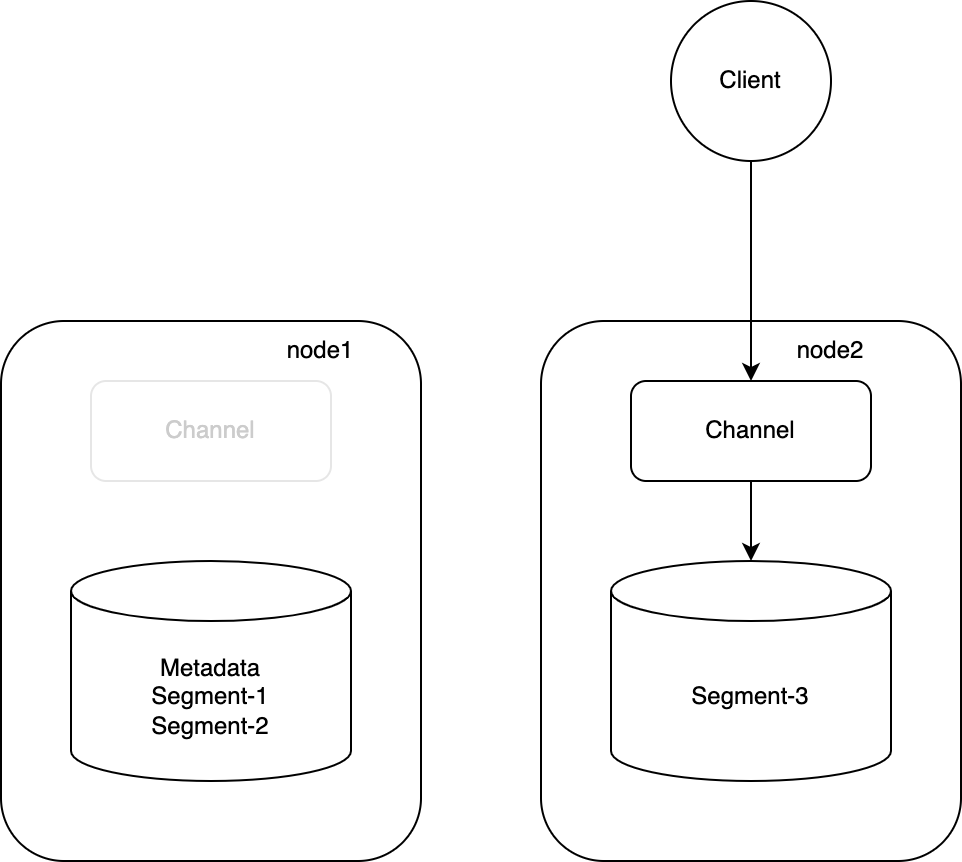
\includegraphics[width=7cm, keepaspectratio]{images/migrating-client.png}
    \end{center}
\end{frame}

\begin{frame}
    \frametitle{Challenge 2: Migrating clients}
    \framesubtitle{Approach 1: Two step assemble}

    \begin{center}
        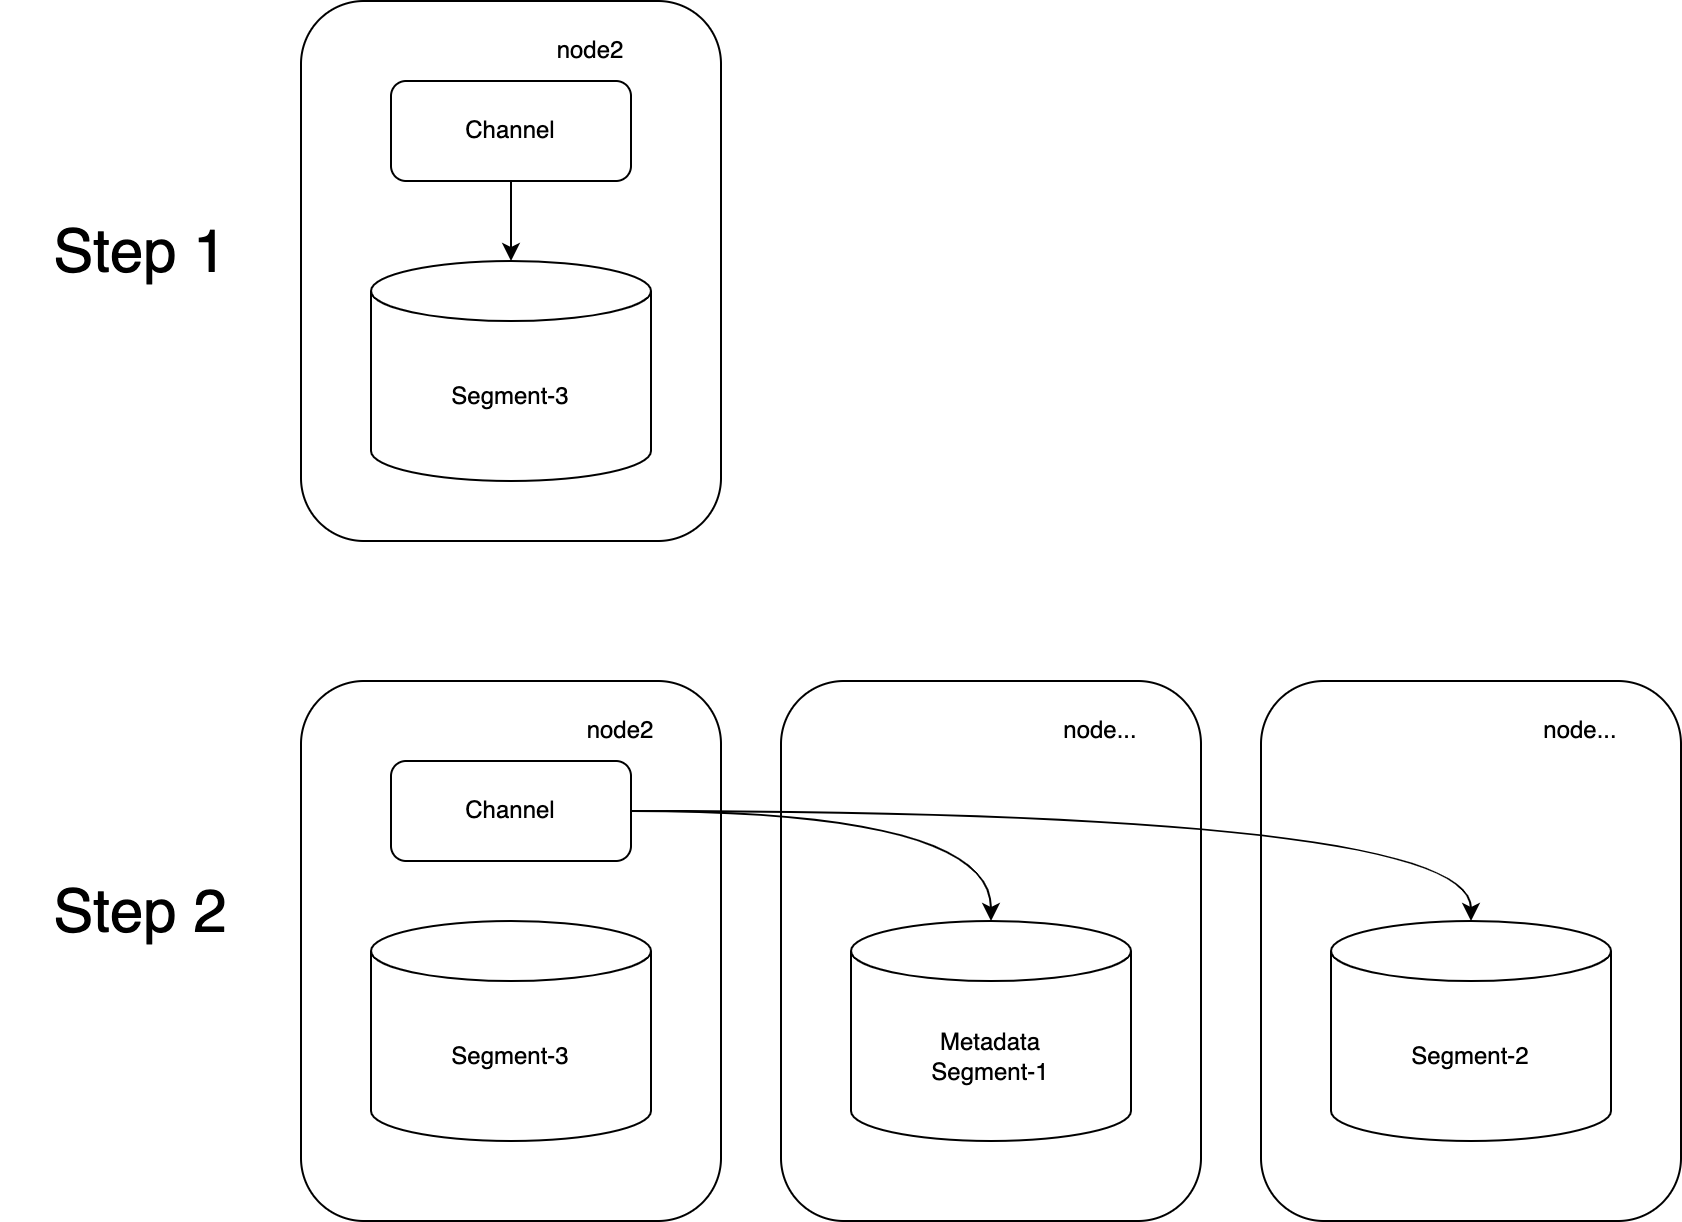
\includegraphics[width=7cm, keepaspectratio]{images/assemble-1.png}
    \end{center}
\end{frame}

\begin{frame}
    \frametitle{Challenge 2: Migrating clients}
    \framesubtitle{Approach 2: Replicated data}

    \begin{center}
        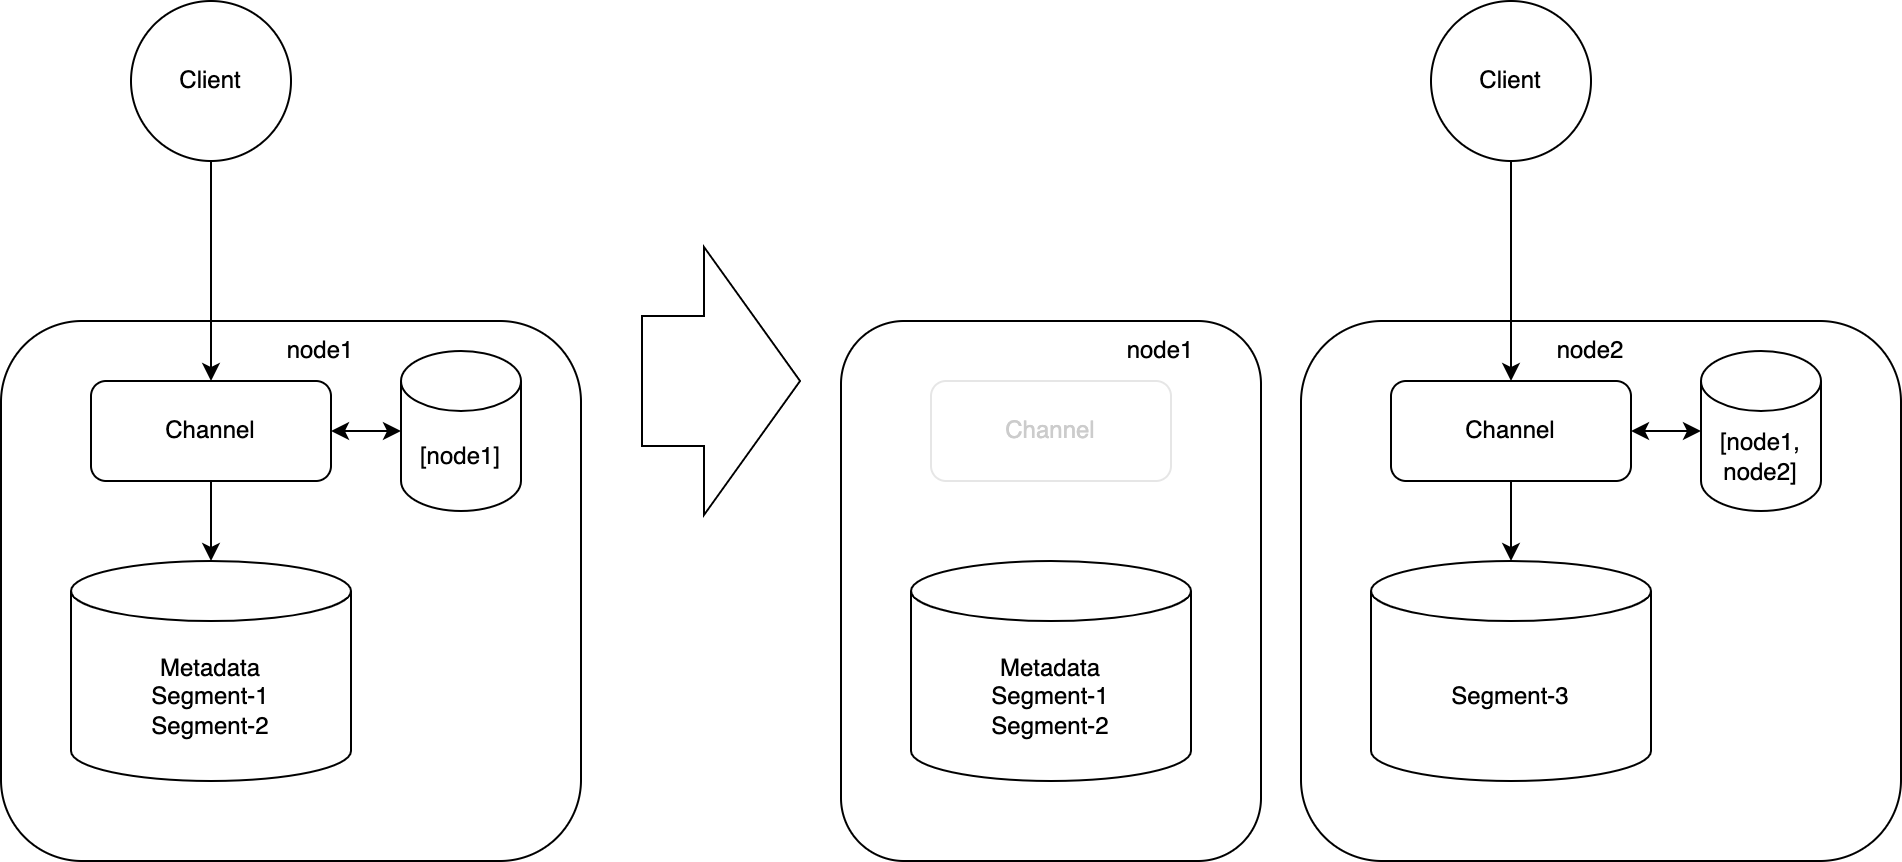
\includegraphics[width=7cm, keepaspectratio]{images/replicated-data.png}
    \end{center}
\end{frame}

\begin{frame}
    \frametitle{Challenge 2: Migrating clients}
    \framesubtitle{Approach 2: One step assemble}

    \begin{center}
        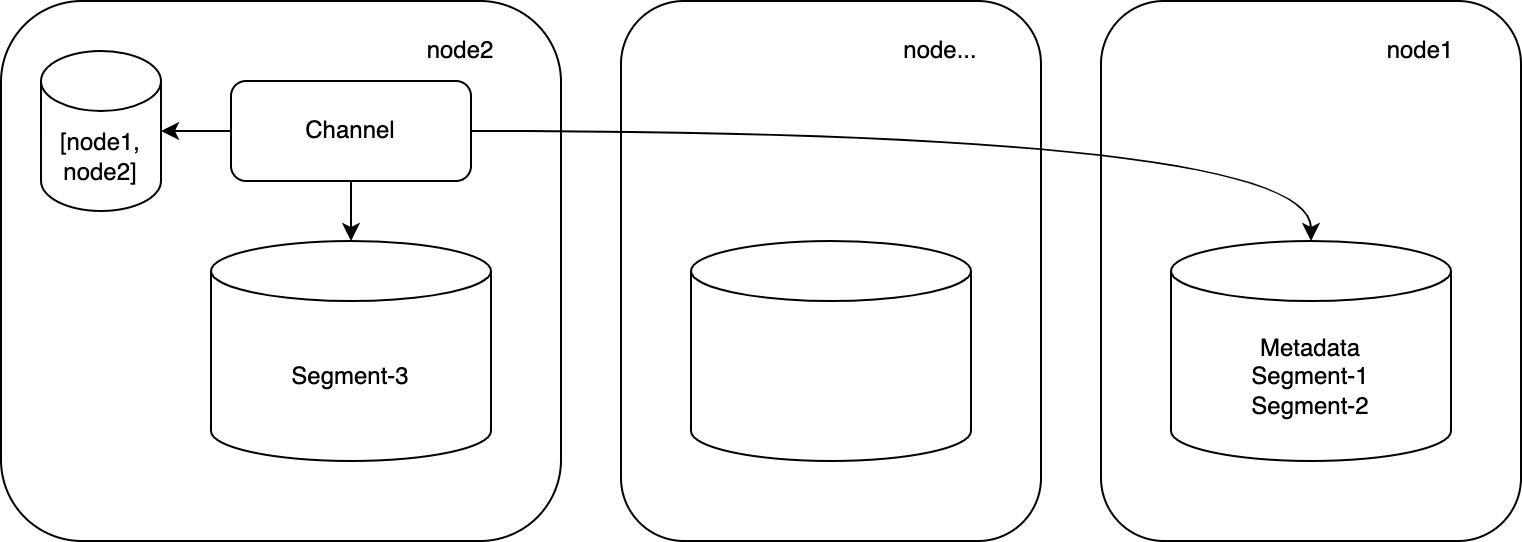
\includegraphics[width=7cm, keepaspectratio]{images/assemble-2.png}
    \end{center}
\end{frame}

\begin{frame}
    \frametitle{Challenge 3: Long-running operations}
    \framesubtitle{\lstinline{PUBLISH} handling}

    \begin{center}
        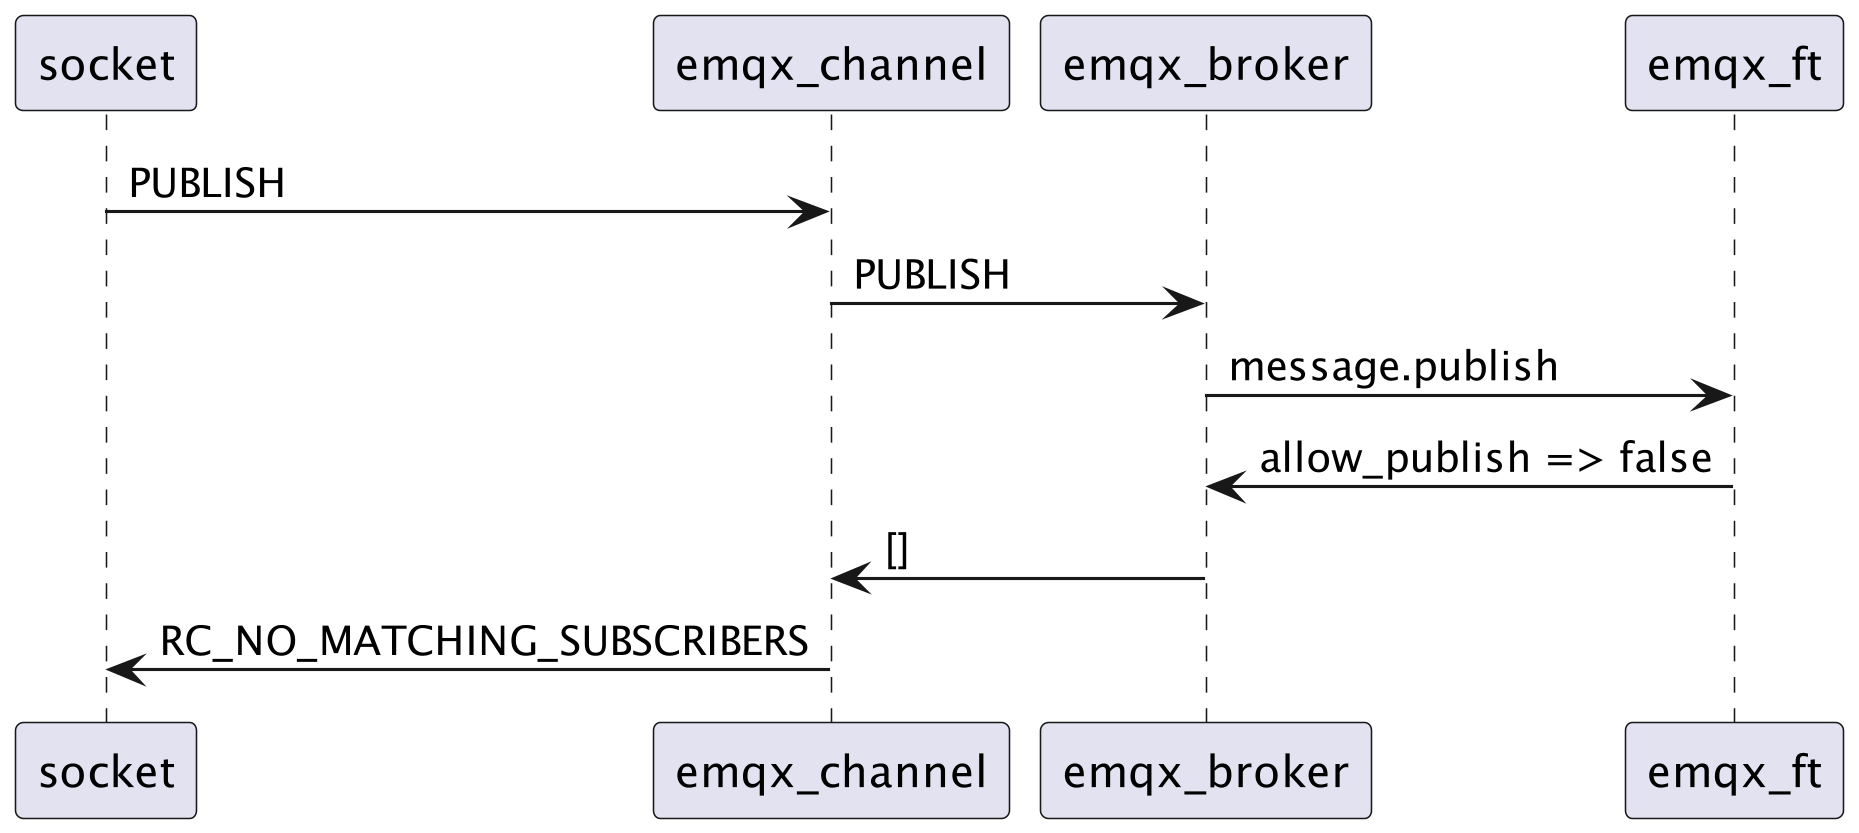
\includegraphics[width=7cm, keepaspectratio]{images/sync-publish.png}
    \end{center}
\end{frame}

\begin{frame}
    \frametitle{Challenge 3: Long-running operations}
    \framesubtitle{\lstinline{PUBLISH} handling: Desired}

    \begin{center}
        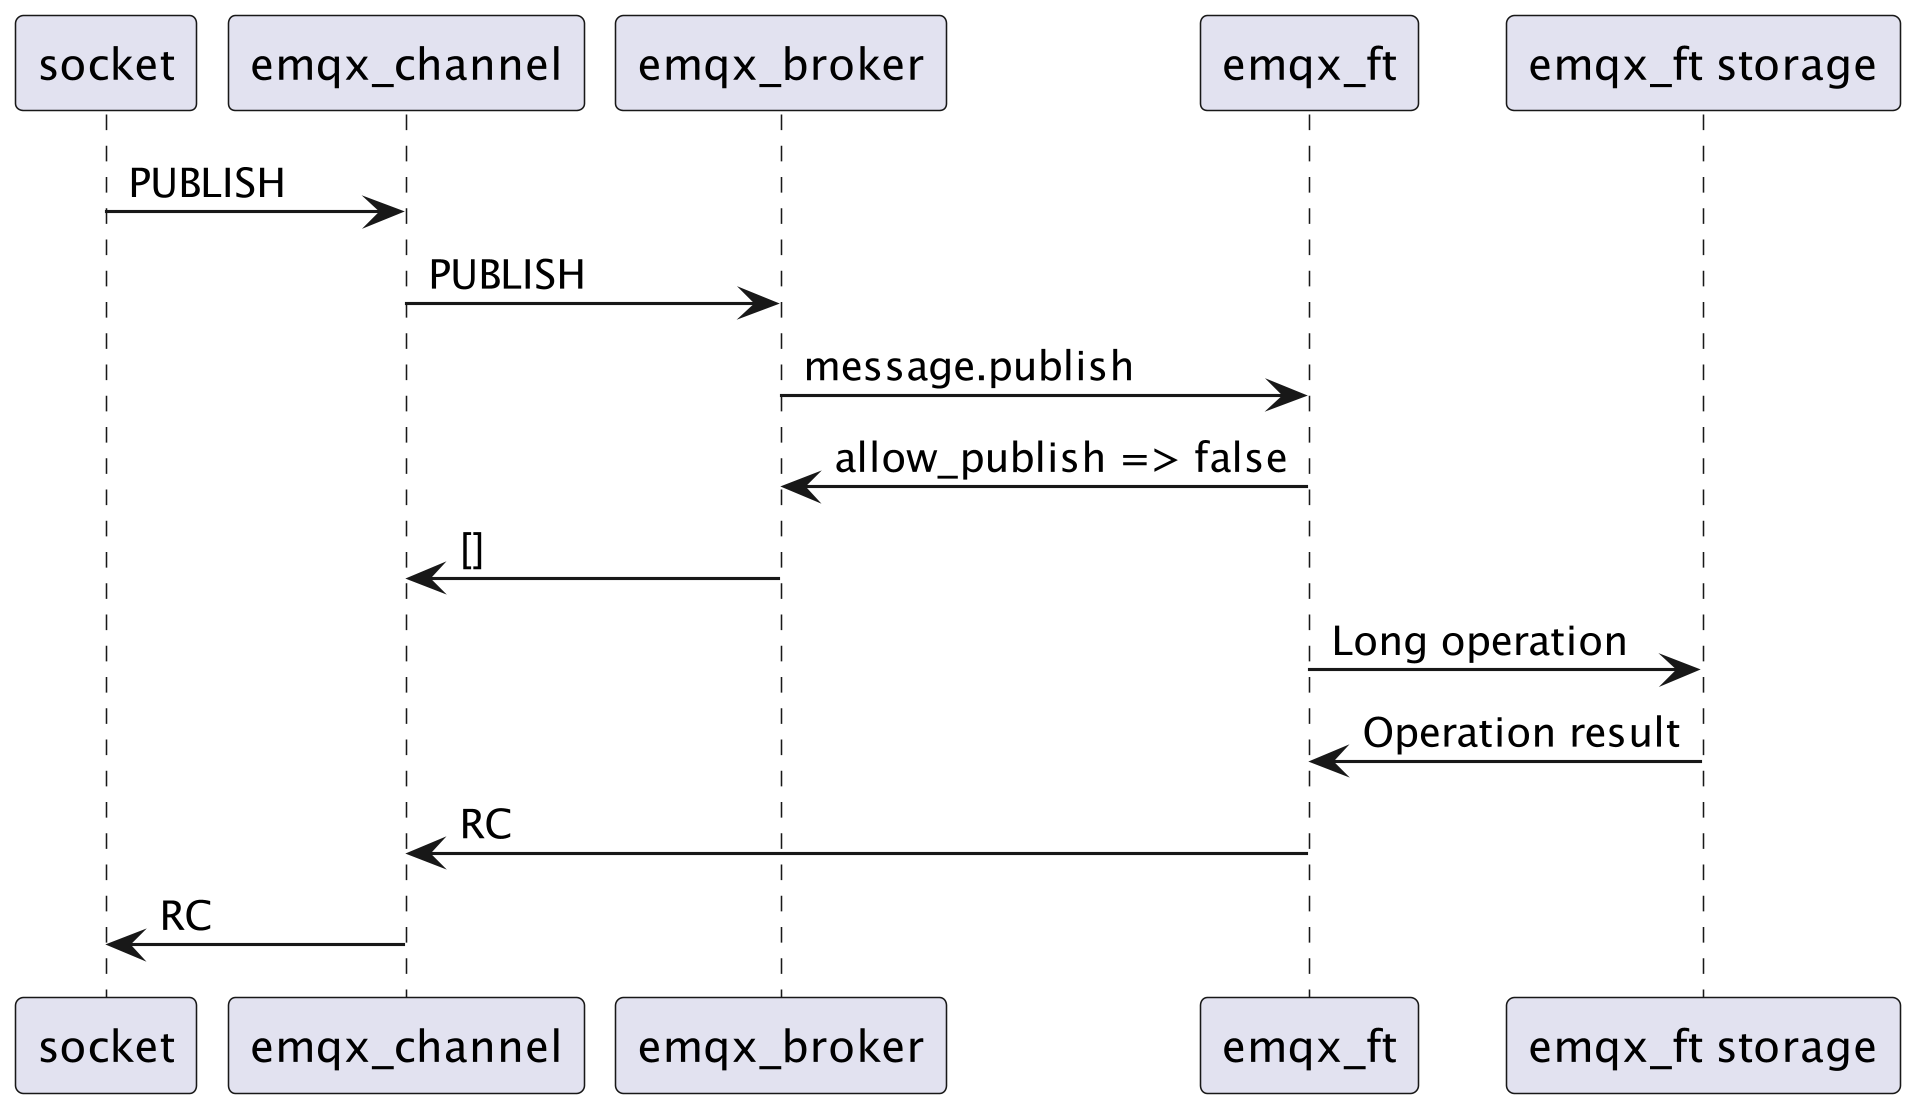
\includegraphics[width=7cm, keepaspectratio]{images/async-publish-needed.png}
    \end{center}
\end{frame}

\begin{frame}
    \frametitle{Challenge 3: Long-running operations}
    \framesubtitle{\lstinline{PUBLISH} handling: Implemented}

    \begin{center}
        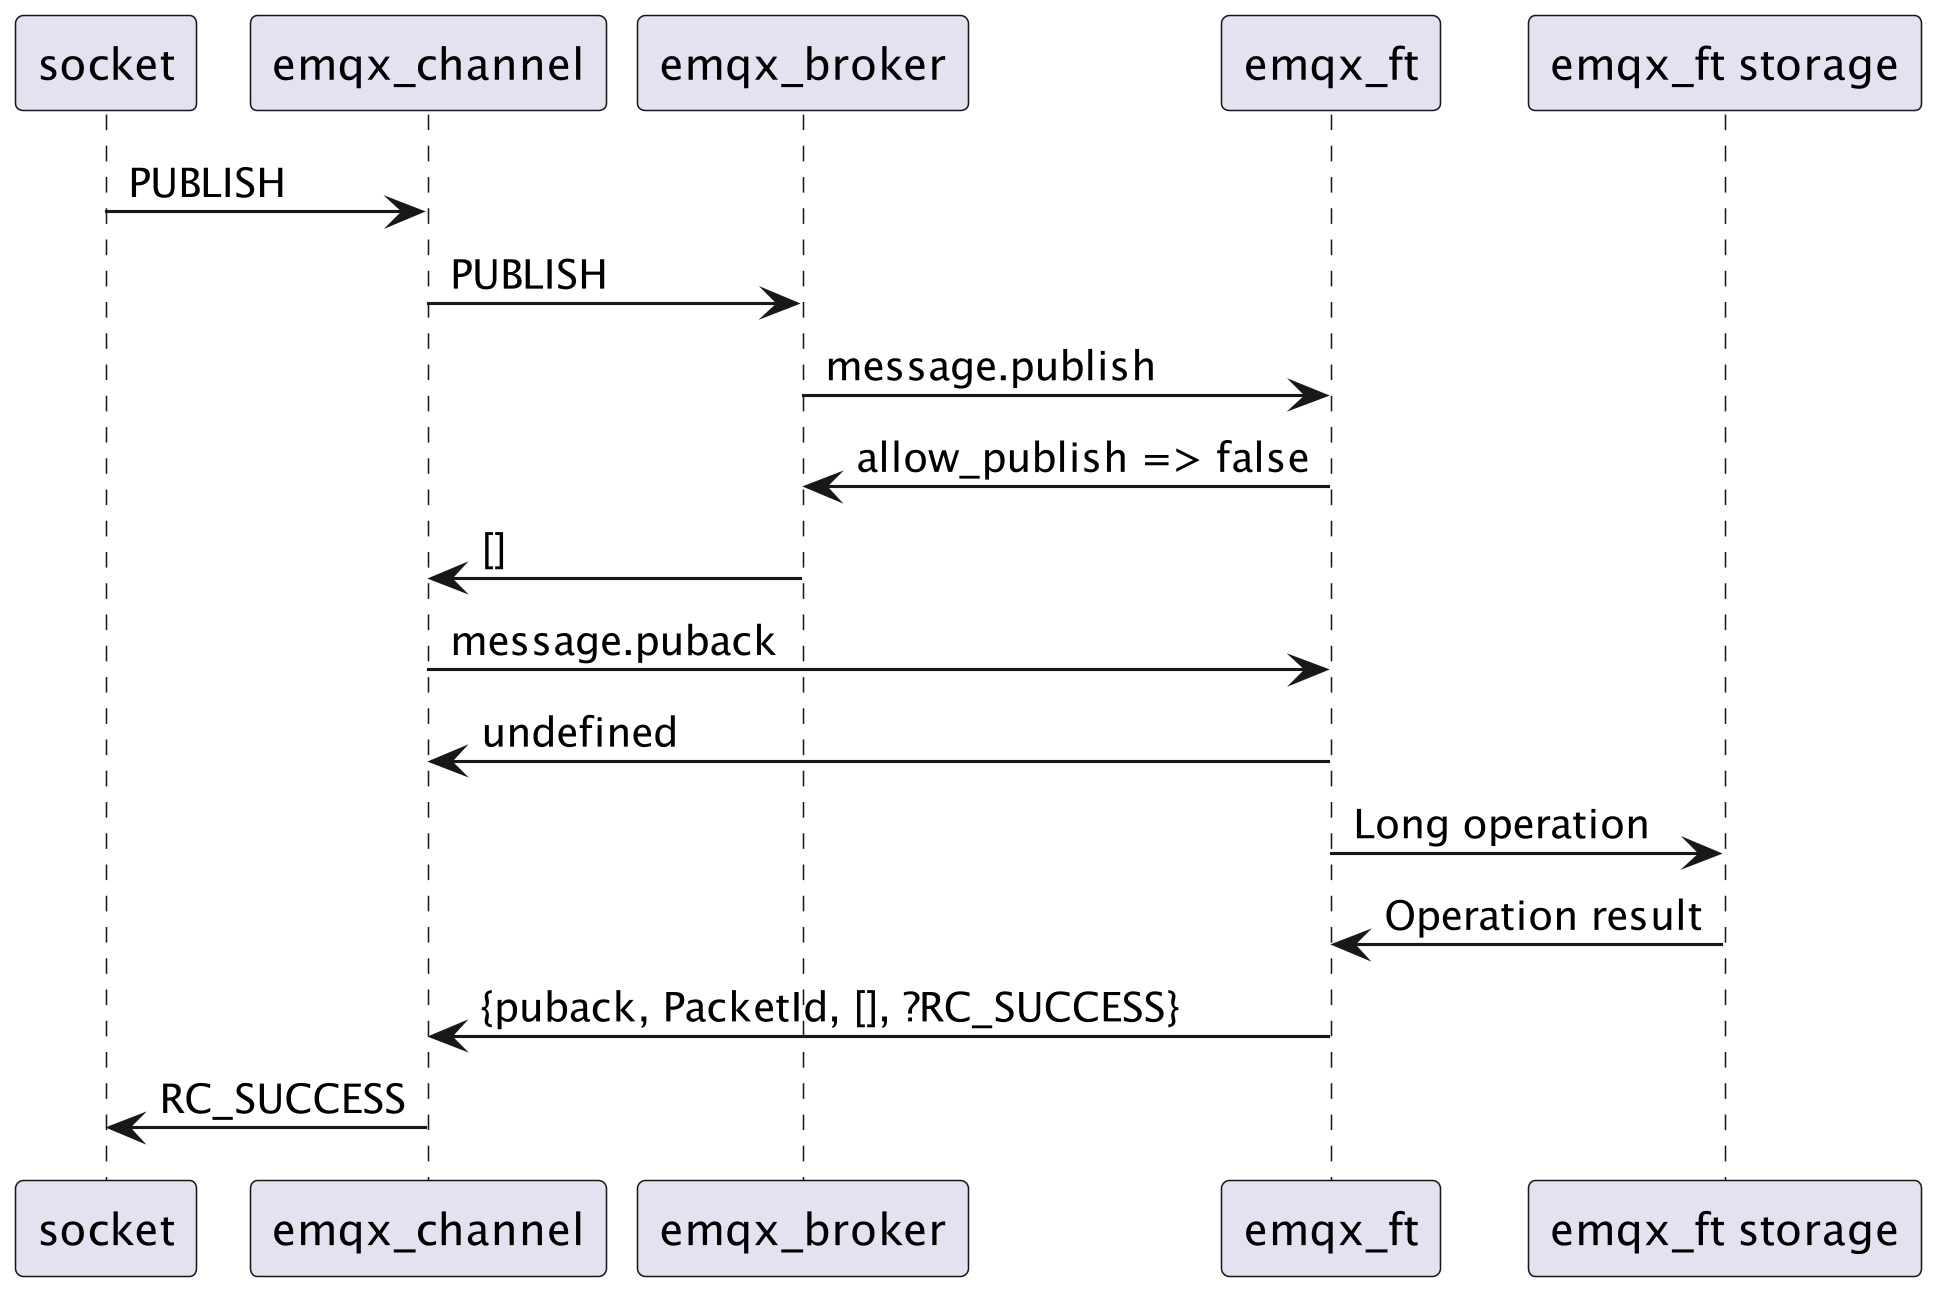
\includegraphics[width=7cm, keepaspectratio]{images/async-publish-implemented.png}
    \end{center}
\end{frame}

\begin{frame}
    \frametitle{File Transfer}
    \framesubtitle{TODO: Must have}
    \begin{itemize}
        \item Ensure reliability of the storage part (testing, IO error handling, GC, etc.)
        \item Ensure reliability of the MQTT part (testing, MQTT client scenarios handling, etc.)
        \item Consider making all FT methods async, not only \lstinline{fin}
        \item Improve observability (API)
    \end{itemize}
\end{frame}

\begin{frame}
    \frametitle{File Transfer}
    \framesubtitle{TODO: Should have}
    \begin{itemize}
        \item Implement quotas: storage, bandwidth, tps
        \item Implement metrics
    \end{itemize}
\end{frame}

\begin{frame}
    \begin{center}
        Thank you!
    \end{center}
\end{frame}

\end{document}
